\newSec[ControlPosAccel]{Erzeugung von Posen aus Beschleunigungsdaten}{2}




\newSec[ControlPosAccelCalc]{Berechnung}{3}


\missing[doppelt integieren]






\newSec[ControlPosAccelDisturb]{Störgrößen}{3}
Nachfolgend soll auf Einflüsse der Messung auf die Qualität der ermittelten Pose eingegangen werden. Hierzu werden verschiedene Störgrößen am Beispiel eines Szenarios betrachtet und mögliche Gegenmaßnahmen gezeigt.


\missing[Hier den Inhalt aus der Excel-Mappe Signalverarbeitung]



\newSec[ControlPosAccelSzenario]{veranschaulichendes Szenario}{4}
Im gewählten Szenario wir die z-Achse \bzw\ Flughöhe als Beispiel betrachtet. 
Die Kurve setzt sich aus idealisierten Teilstücken zusammen (siehe \refImg{fig:SzeneOrigin}, oben):
\begin{itemize}
\item Initialisierung: horizontale Gerade
\item Abflug: negativer Cosinus (1/2 Schwingung)
\item Schweben: horizontale Gerade
\item Landung: zwei entgegengesetzte Parabeln\footnote{Die Parabeln sind so angeordnet, dass der Berührungspunkt zeitlich in der Mitte der Landungsphase liegt. Da die Parabeln einen identischen Streckfaktor besitzen, entspricht der Übergang zwischen den Parabeln einer knickfreien Kurve.}
\item Abschalten: horizontale Gerade
\end{itemize}


\begin{figure}[ht!]
\vspace{0.25cm}
\begin{center}
\fbox{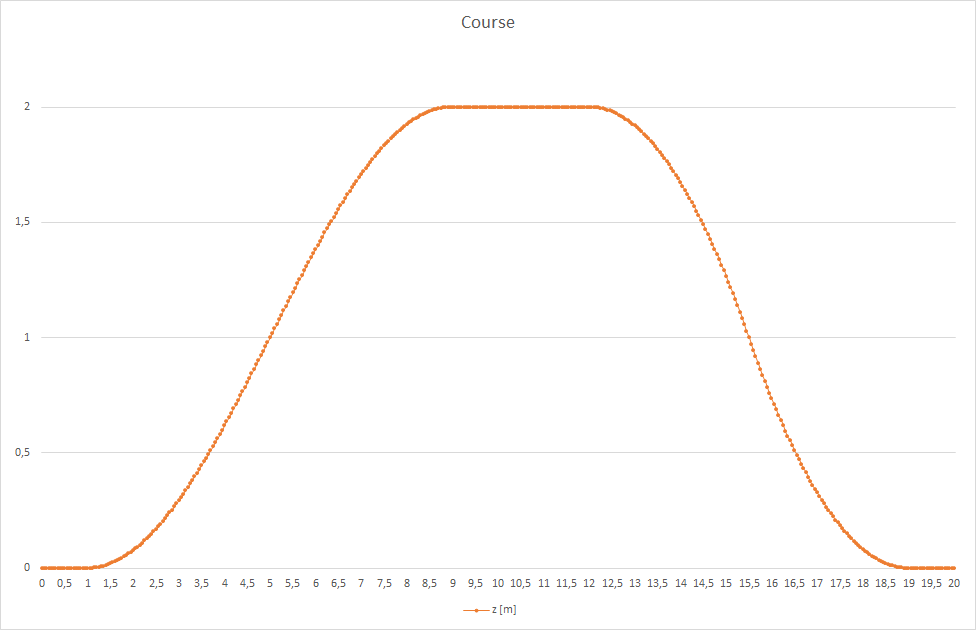
\includegraphics[width=15cm]{Pictures/Szenario Origin z.png}}
\fbox{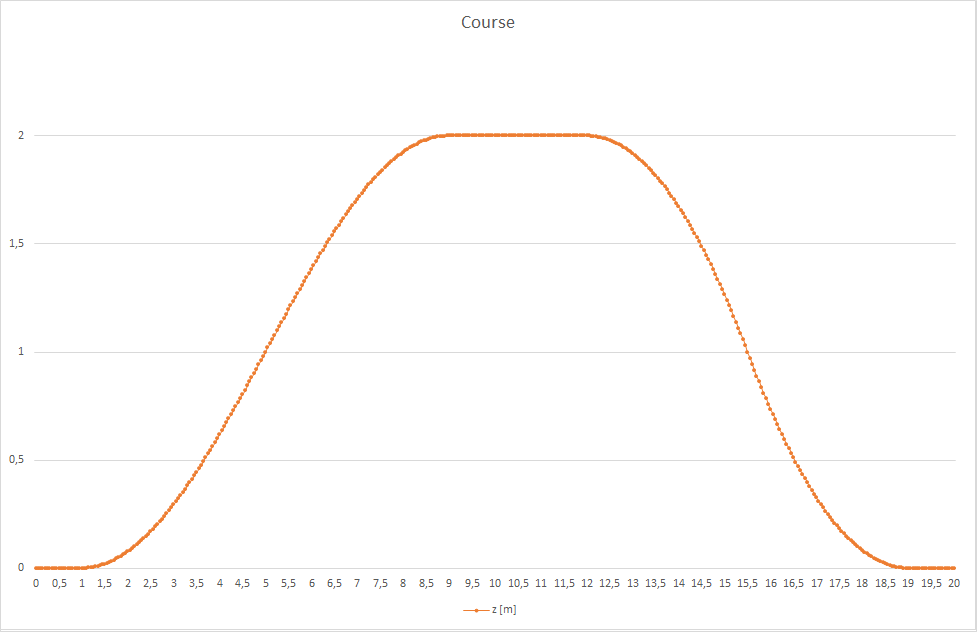
\includegraphics[width=15cm]{Pictures/Szenario Origin az.png}}
\caption{Originalkurve des Szenarios}
\label{fig:SzeneOrigin}
\end{center}

\vspace{0.25cm}
In \refImgShort{fig:SzeneOrigin} sind der idealisiete Höhneverlauf (oben) und die daraus abgeleitete Beschleunigung (unten) aufgetragen.
\end{figure}


Die Beschleunigungsdaten wurden aus der genannten Kurve mittel zweifacher zeitdiskreter Differentation gebildet (siehe \refImg{fig:SzeneOrigin}, unten).

Durch dieses Vorgehen ist sichergestellt, dass ein Vergleich zwischen original Kurve und den rekonstruierten Verläufen gebildet werden kann. In diesem Zusammenhang wurde sichergestellt, dass eine Rekonstruktion ohne aufgeprägte Störgrößen möglich ist.







\newSec[ControlPosAccelNoise]{Rauschen}{4}

\missing[Messfehler, Abweichungen von AD Wandlern, Vibration (bei Beschleunigungsmessdosen)]




\begin{figure}[ht!]
\vspace{0.25cm}
\begin{center}
\fbox{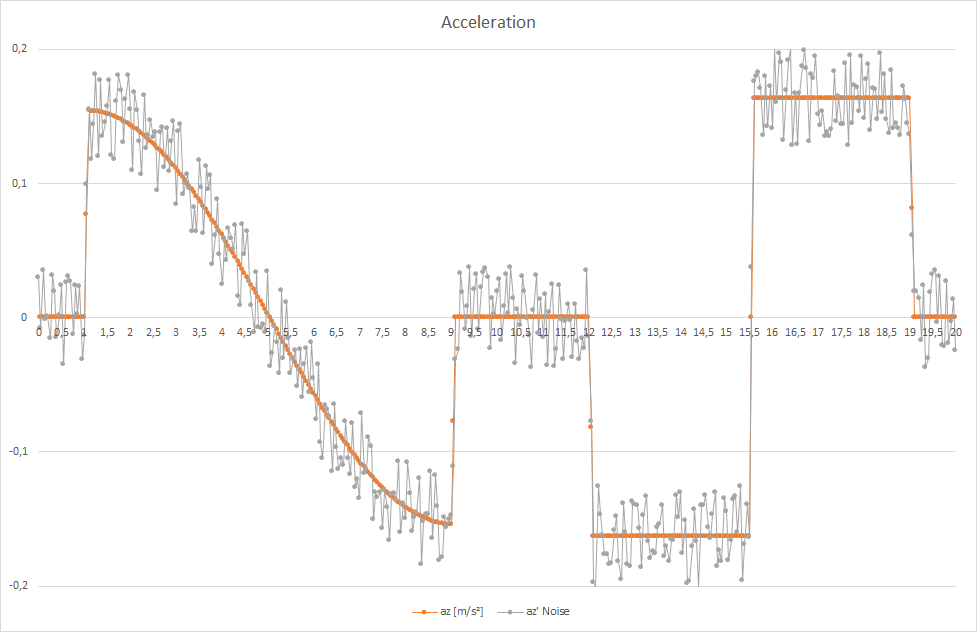
\includegraphics[width=12cm]{Pictures/Szenario Noise az.png}}
\fbox{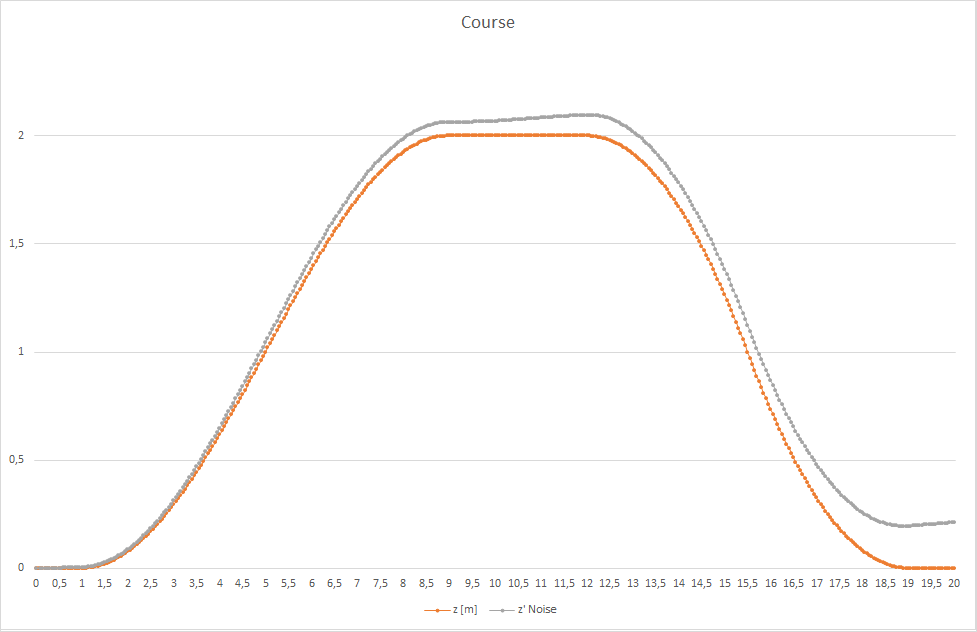
\includegraphics[width=12cm]{Pictures/Szenario Noise z.png}}
\caption{Einfluss von Signalrauschen}
\label{fig:SzeneNoise}
\end{center}

\vspace{0.25cm}
\end{figure}


\newSec[ControlPosAccelOutlier]{Ausreißer}{4}


\begin{figure}[ht!]
\vspace{0.25cm}
\begin{center}
\fbox{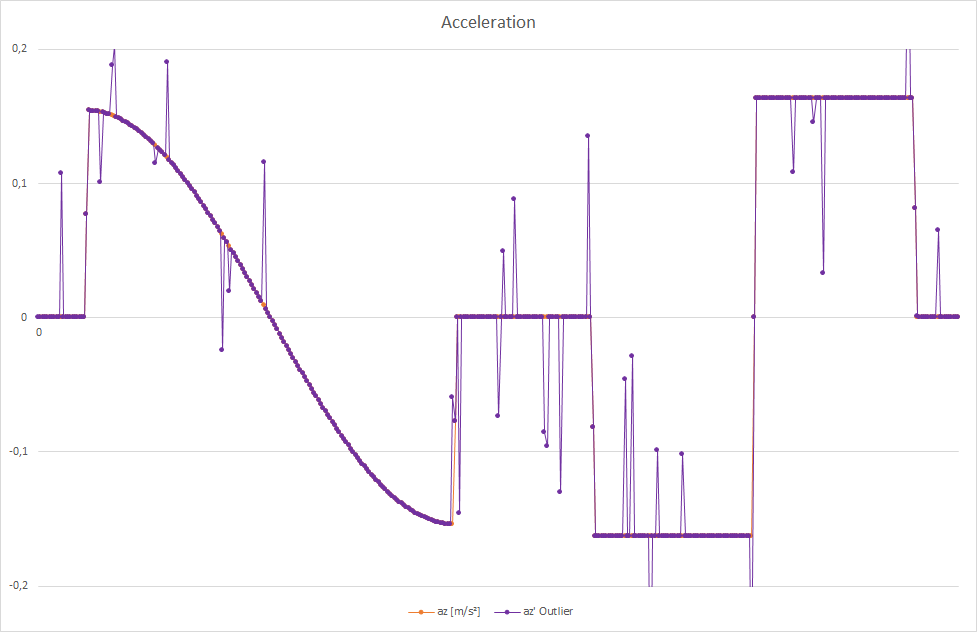
\includegraphics[width=12cm]{Pictures/Szenario Outlier az.png}}
\fbox{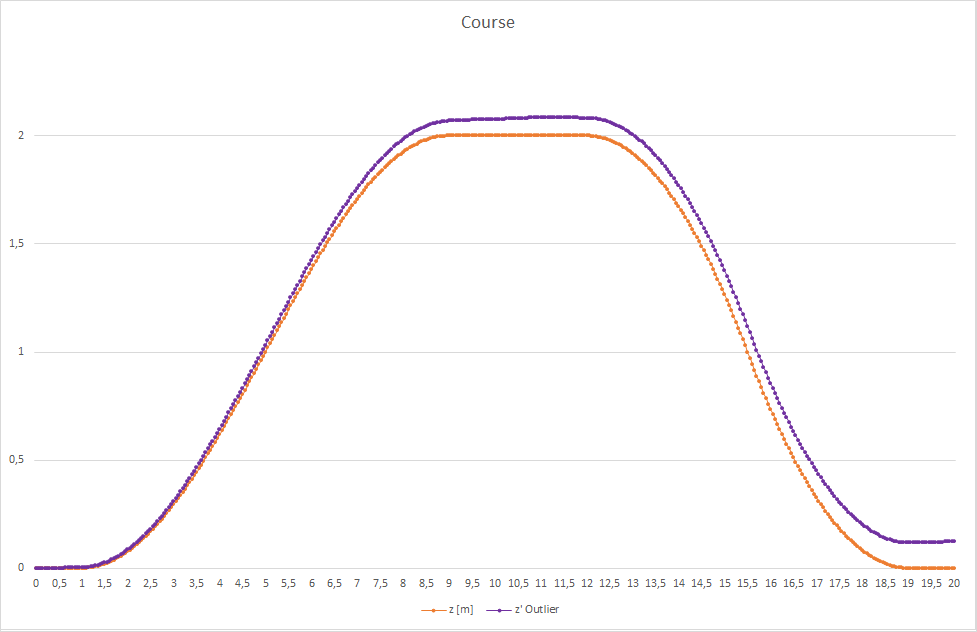
\includegraphics[width=12cm]{Pictures/Szenario Outlier z.png}}
\caption{Einfluss von Ausreißern}
\label{fig:SzeneNoise}
\end{center}

\vspace{0.25cm}
\end{figure}





\newSec[ControlPosAccelOffset]{konstante Nullpunkt-Abweichung}{4}





\begin{figure}[ht!]
\vspace{0.25cm}
\begin{center}
\fbox{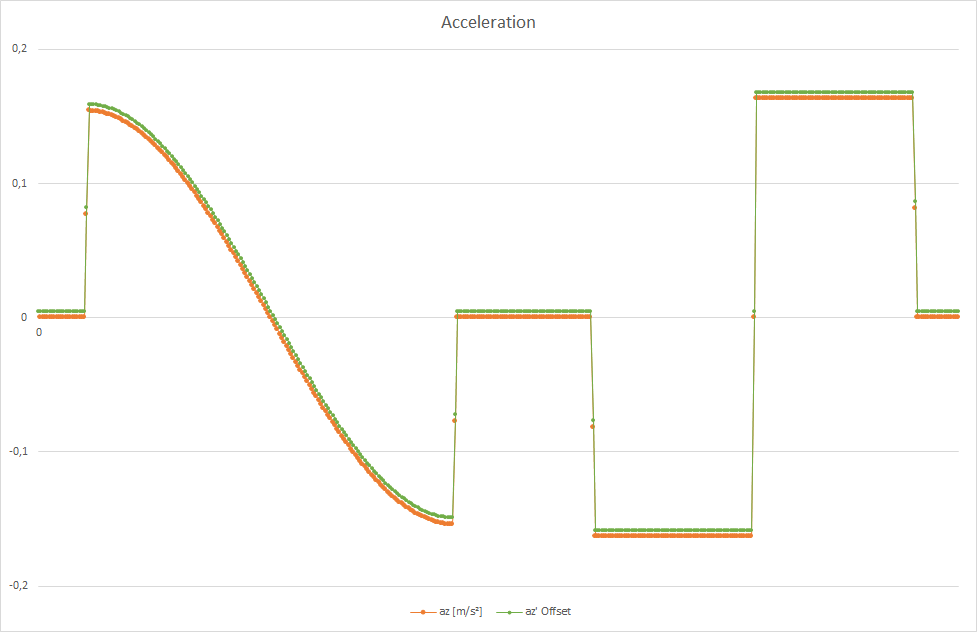
\includegraphics[width=12cm]{Pictures/Szenario Offset az.png}}
\fbox{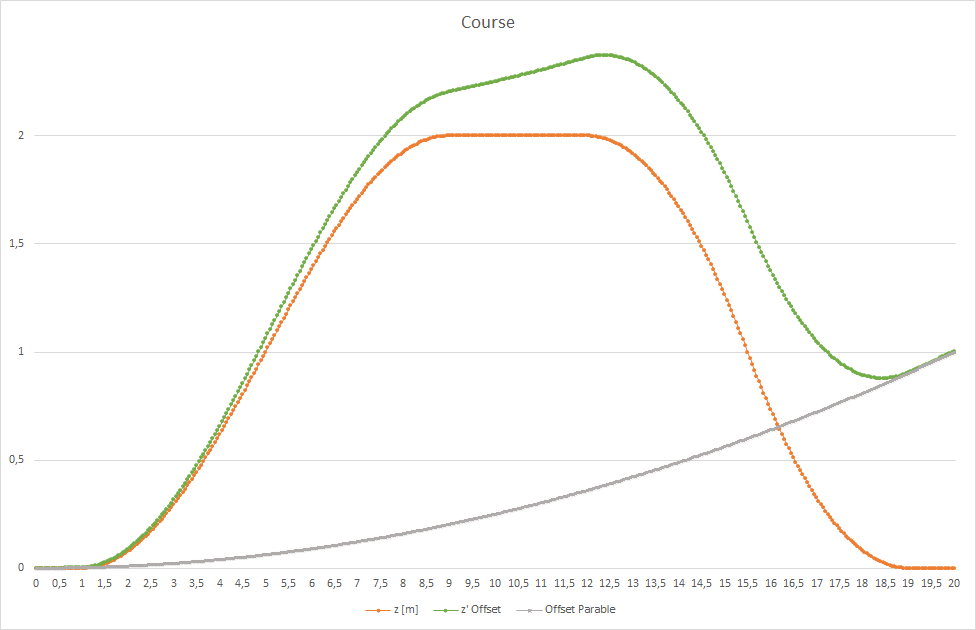
\includegraphics[width=12cm]{Pictures/Szenario Offset z.png}}
\caption{Einfluss von konstanter Nullpunkt-Abweichung}
\label{fig:SzeneNoise}
\end{center}

\vspace{0.25cm}
\end{figure}













